\chapter{Introduction}

% new methods, new large data. 

Since the first sequencing and assembly of the human genome~\cite{FirstHumanGenome}, this confluence of chemistry, general and molecular biology, genetics, and medicine bore a new field of computational biology --- and it continues to grow and present new challenges which stem from the number and complexity of the hypotheses it generates and sheer volumes of data to be analyzed simultaneously. Sequencing technologies have vastly improved since then resulting in a sharp descrease in costs which, in turn, helped sequencing machines become a commonplace in many research centers, forensic labs, and hospitals. Advances in DNA sequencing coincided with a rapid development of other high-throughput techniques that aimed to capture interactions between proteins~\cite{yeast2hybrid,TAPMS}, dependencies between metabolites, genes, and gene products~\cite{ChipSeq,GeneKnockouts}, rates of gene transcription~\cite{RNAseq} and protein translation~\cite{riboseq} XXX offering enough data to correlate the inner workings of the cells.

% Noise, large volume, many alternative solutions -- ways to extract insights automatically and visualize at scale. Visualization as important as the methods that analyze the data -- one helps to generate hypotheses and the other -- to test them.

% GCN -- examples of complex data. GCN
These new data provided a first glimpse into how organisms operate on a molecular level on a global scale --- the scale of thousands of genes and proteins at a time, along with their complex interactions and dependencies. For example, microarray panels~\cite{microarray} and, later, RNA-seq~\cite{RNAseq} experiments measure gene expression for large numbers of genes simultaneously; these measurements serve as a snapshot of the system under specific conditions at a particular time. The measurements taken under different conditions --- e.g. prior and after administering a drug to a cell culture --- can be compared to each other and point to genes for which the expression levels change significantly between the two conditions. Such \textit{co-expressed} genes may belong to the same drug response pathway and we can start building a co-expression network where nodes are the genes in question and edges connect genes that display a co-expression relationship. These co-expression relationships can be further refined as we repeat the experiment and observe the same cell culture under other conditions. We now can mine the resulting gene co-expression network (GCN) for groups of genes that were consistently co-expressed --- such genes are putatively controlled by the same cellular mechanism and may perform the same function in the cell. We can further use these strongly related groups of genes to annotate those genes for which the function is not yet known by considering the functional annotations of its neighbors.

% XXX PPIs
Similarly, protein-protein interaction networks (PPIs) can be used to find groups of interacting proteins --- protein complexes where proteins interact physically or perform the same function and participate in the same pathway. In PPI networks, nodes represent the individual proteins, and two proteins are connected by an edge if the proteins interacted. In a yeast two-hybrid (Y2H) experiment~\cite{yeast2hybrid}, the protein interaction is observed when the two proteins bind together and form a transcription factor thus causing a downstream signalling gene to express. Protein interactions obtained through the tandem affinity purification (TAP) method capture whole protein complexes; when TAP step is coupled with mass spectrometry (MS), researchers can discern the individual proteins comprising the complex. Like GCNs, PPI networks contain on the order of thousands of nodes and tens to hundreds of edges~\cite{citeAThalsMain,someEcoliOrYeast}. The progress towards the full proteome of a species: about a decade later after the publication of the TAP-MS protocol, about one third of proteins for a model organism \textit{Arabidopsis thaliana} remained uncharacterized~\cite{cite62}. PPI networks generated through these high throughput methods were then used to assign function to novel proteins. the introduction Multiple algorithms for clustering the network are available~\cite{} that find highly connected subsets of proteins; with downstream methods aiming at inferring function, cellular localization, or the biological process the novel proteins are part of. 

However, identifying such groups of genes or proteins is a non-trivial problem. The classical graph clustering algorithm that seeks to maximize network modularity by separating nodes into non-overlapping groups~\cite{modularity} is an NP-hard problem~\cite{modularityNPhard}. Multiple alternative approaches~\cite{PPIclustering} were developed, especially for PPI networks, and not surprizingly they produce different results on the same input data. Even running the same algorithm on the same data with different tie breaking policies may produce different results each time. The trick is that neither of these clusterings is wrong, and all of them are a view of the data from a different angle. We must consider them all at once to be able to say confidently that these genes were co-expressed or these proteins formed a functional complex. In this thesis, we discuss different metrics for comparing such clustering results and present a workflow that allows to systematically analyze such results simultaneously. We present an approach that finds the most consistently clustered groups of nodes and demonstrate the effectiveness and the need for such an approach by analyzing nine clusterings of protein interaction network of a model organism \textit{Arabidopsis Thaliana}. XXX cite Saket's study on multiple network clusterings w/ modularity and another guy on multiple hierarchical clusterings.

% Analysis methods developed for such complex data would produce solutions that were not necessarily stable or unique, and often, other alternative optimal and near-optimal solutions would be just as valid and just as informative as a single solution obtained under different parameters. Alternative solutions are especially important to consider when working with noisy data such as when looking to identify plausible protein complexes~\cite{VanDongen2000} and groups of genes that act in concert, to infer protein function and to annotate new data based on existing ontologies. We discuss approaches to automatically analyze and visualize such ensembles of solutions.

%For example, proteins rarely function alone and tend to physically interact with other proteins through electrostatic forces forming a stable protein complex. tapMS and  interaction networks capture these interactions, for example, capture . XXX add more of a bridge between noisy data and multiple solutions; along w/ a need to analyses these solutions in concert and systematically. Describe PPI data and what kinds of questions it could answer when all interactions are taken together. Mention gene/protein annotations databases -- used in analyses to assign unknown functionl infer missing pathways, protein interactions, whole complexes.

% Often, the insights were hidden under the layers of experimental noise and natural variation; with hypotheses testing hindered by large data volumes. Analysis methods developed for such complex data would produce solutions that were not necessarily stable or unique, and often, other alternative optimal and near-optimal solutions would be just as valid and just as informative as a single solution obtained under different parameters. Alternative solutions are especially important to consider when working with noisy data such as when looking to identify plausible protein complexes~\cite{VanDongen2000} and groups of genes that act in concert, to infer protein function and to annotate new data based on existing ontologies. We discuss approaches to automatically analyze and visualize such ensembles of solutions.

% XXX make multiple solutions a separate paragraph -- give a simpler example for when comparing multiple solutions to a thing is important. discuss the space of alternative solutions -- inexact data, noisy data, random decisions when clustering, breaking the ties -- all leads to multiple, alternative as-good solutions
 
% Visualization as important as the methods that analyse the data -- one helps to generate hypothese and the other -- to test them.

Analysis of complex data, such as PPIs or GCNs, gives us a global perspective on cooperation between proteins and genes, however, to understand the workings of a single complex and its response to stimuli, we would want to consider the network at a local level and observe it over time or under various conditions. XXX give an example of drug absorption, then go on to describe contributions. 
We developed a visualization approach that focuses on local neighborhoods around a single node and tracks topological changes over time. We use a dynamic social network of jazz musicians that captures their interactions over the course of a hundred years, however, the same design principles will easily carry over to a dynamic biological network. The principles used in that visualization --- interactivity, exploration, details-on-demand --- follow HCI principles and apply to dynamic biological networks in equal measure.

% XXX large volume -- compression.

xxx need to establish the need for these topics a little more. add more discussion, stories, motivation for why these ideas are important to consider. add more connection between different pieces.

Large data volumes resulting from high-throughput experiments present yet another, more fundamental challenge. Technical demands for storage and transmission of such data volumes hinder easy exchange of information and the ability to run complex analyses on the data. Traditional compression techniques alleviate the problem of data transfer, but require that data is fully decompressed to perform any analyses and may not exploit domain knowledge about the nature of the data and the way data is going to be used to improve compression ratios. Later in this thesis, we investigate compression methods for one of the most abundant data types in computational biology --- the nucleotide sequences.

% Large data volumes resulting from high-throughput experiments present yet another challenge. To maintain interactivity and to provide useful insights, the software must offer ways to aggregate data and generate an overview without oversimplifying or obscuring the underlying patterns. Since manual inspection is infeasible for large data, the software should offser ways to extract meaningful higher-order motifs. Aggregate structure may speed up  computation as in functional compression XXX

XXX in this thesis, we used a v ariety of tools to address scientific needs for large biological data analysis. Importance of methods. Importance of visualization.

This underlines the need for visualization when working with data. A single solution may be persuasive unless you see/or somehow else familiarize yourself w/ the whol space of solutions. Visualization relies on human intutition to help see that.

XXX add more of a bridge into visualization -- numerical analysis alone may be misleading. visualization can speed up hypothesis generation and testing -- citation? to insight faster than considering some of the standard. in this thesis, we consider visualization as a means to observe network dynamics over time and to analyse alternative solutions -- areas where coming up with a hypothesis is a complex task.

%%
%% Anscombe's quartet 
%%
\begin{figure}[ht]
  \centering
  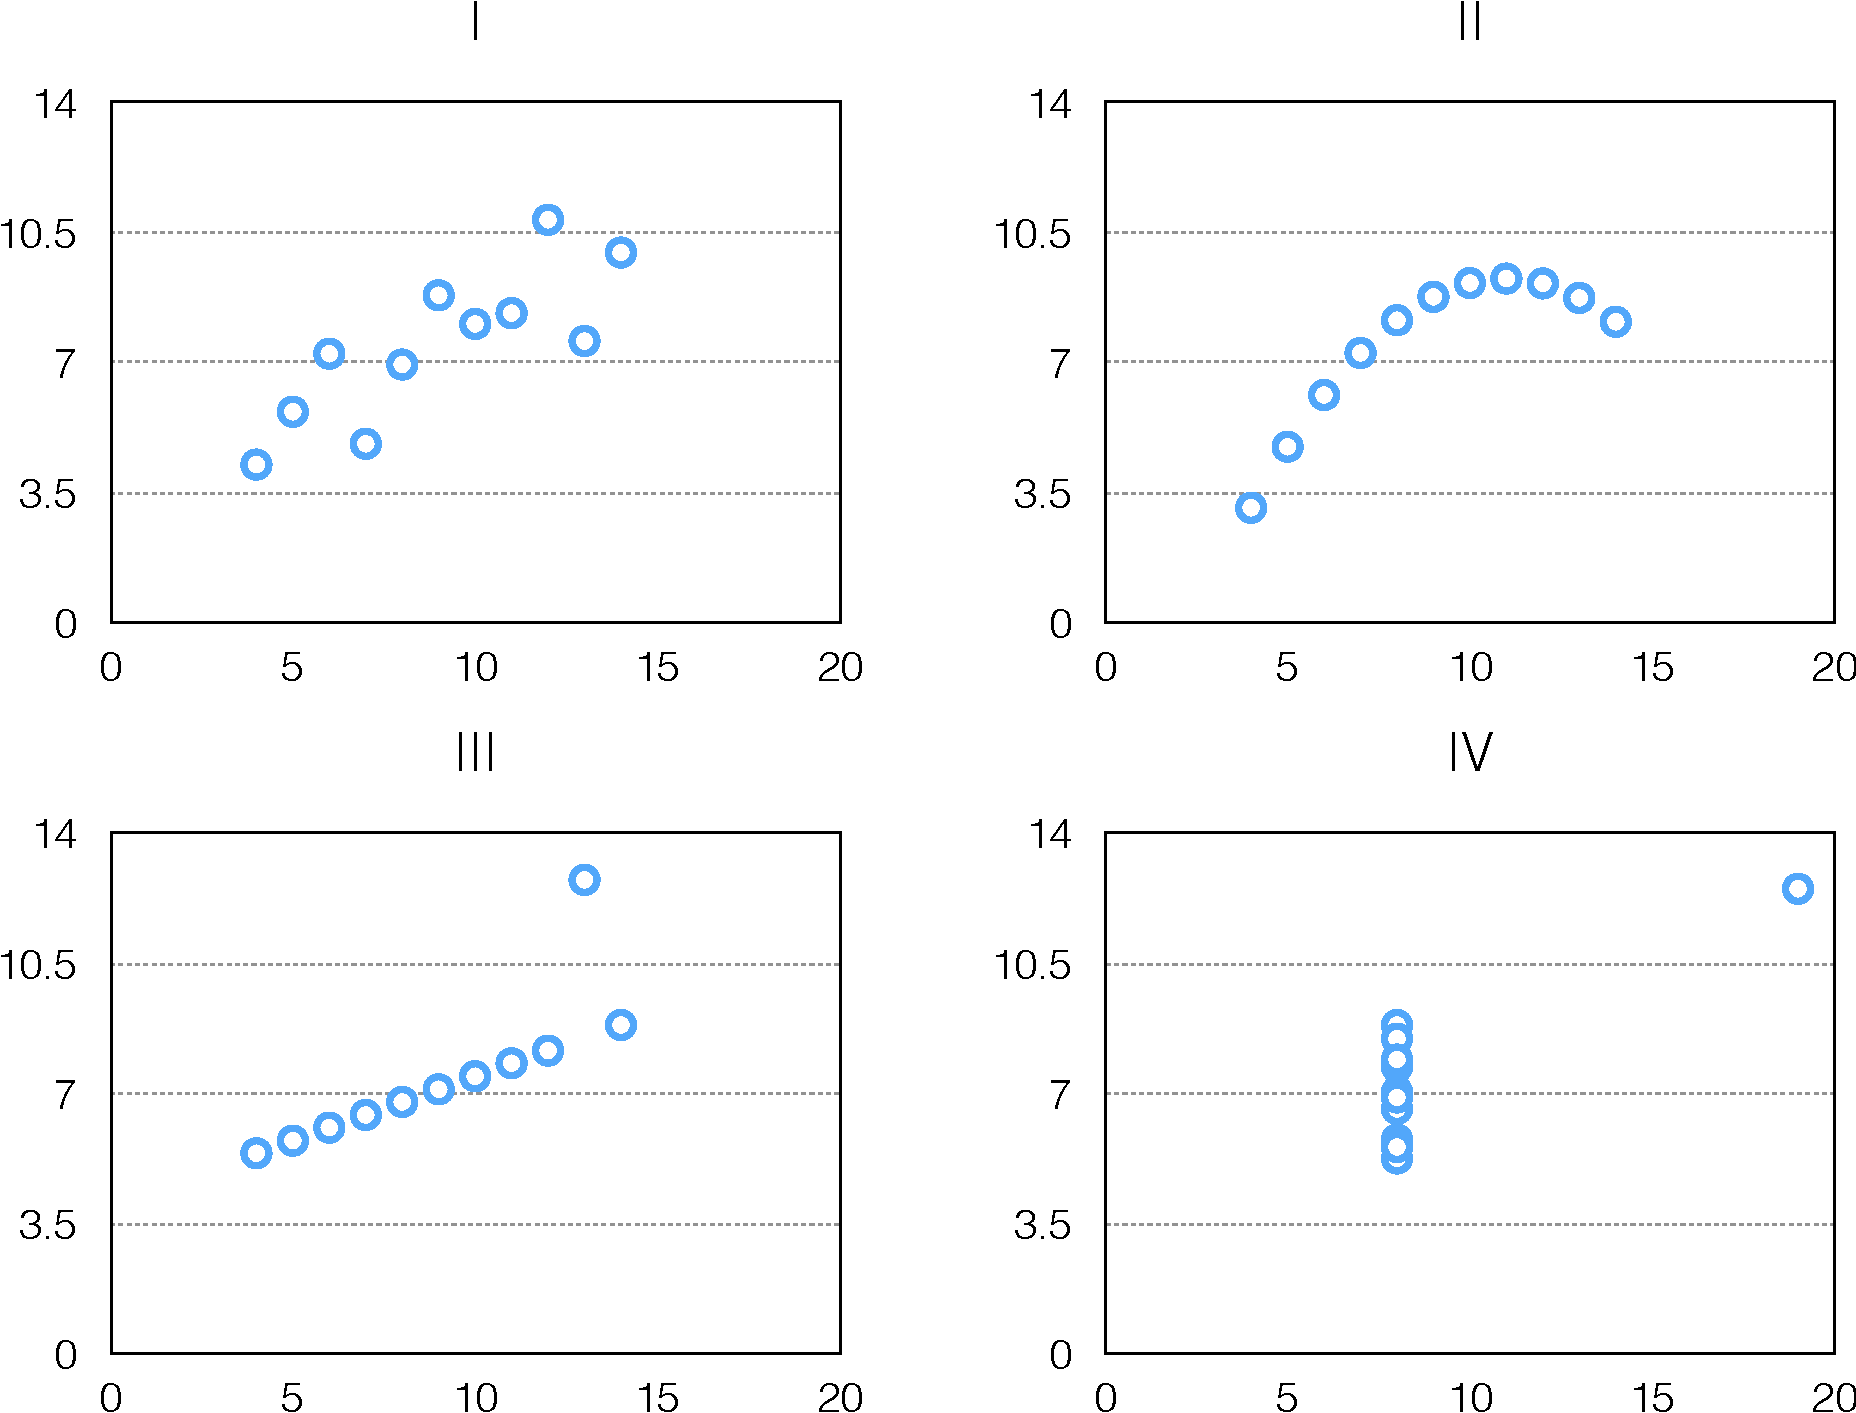
\includegraphics[width=0.8\linewidth]{figures/anscombes_quartet}
  \caption{\textbf{Anscombe's quartet.} Statistician F. Anscombe constructed these four data series to stress the importance of plotting the data before computing its summary statistics. These four sets of data points are indistinguishable when considering their $x$ and $y$ mean, variance, correlation, and linear regression, yet are strikingly different when visualized.}
  \label{fig:intro:anscombe}
\end{figure}


Visualization is an important first step when working with a new set of data as it provides the means to assess the overall shape of the data, its distribution, and to detect outliers. Anscombe's quartet~\cite{anscombe} succinctly demonstrates the importance of viewing the data before analyzing it: four datasets have the same $x$ and $y$ mean and variance, Pearson's correlation and fit the same regression line, yet are strikingly different (Figure~\ref{fig:intro:anscombe}). We see visualization as the means to generate new hypotheses that are then tested and validated through domain-specific algorithms and statistical models.
% Simiarly, complex high-dimensional biological data requires novel visualization approaches that provide an overview of the data along with more detailed and focused displays.

% XXX Russell: this is a good general introduction, but more of a literature review of the specific topics you consider below might be appropriate



%%%%%%%%%%%%%%%%%%%%%%%%%%%%%%%%%%%%%%%%%%%%%%%%%%%%%%%%%%%%%%%%%%%%%%%%%%%%%%%
\section{Major contributions}

We outline the problems addressed in this thesis and the specific contributions made while researching these topics:

\begin{itemize}
  \item \textbf{Visualization and inference of stable subsets in ensembles of classifications}

  We develop new and adapt existing visualizations useful for evaluation and comparison of collections of annotations derived from large datasets through various classification and clustering strategies. We integrate these visualizations into a single comprehensive application that allows to perform a variety of analyses on these classification results. We develop algorithms that reorder data in a way that exposes patterns and helps to identify prominent substructures more easily. Our novel algorithm for core finding automatically extracts annotations that are most consistent across all sets of assigned labels. We use our tool to perform a detailed analysis of clusters of protein-protein interactions in \textit{A. thaliana} plant and identify robust cluster cores that are significantly enriched for Gene Ontology~\cite{GeneOntology} terms and can be used in downstream analyses with greater confidence than clusters generated by a single algorithm.

  % \item \textbf{Augmented search in Sequence Read Archive (SRA)}
  % SHARQ

  \item \textbf{Visual exploration of large dynamic networks}

  We propose an egocentric network view as the main visualization to use when  studying large graphs that change over time. We augment the view by developing node and edge glyphs that summarize the interactions taking place before and after the current point in time. We develop a node ordering algorithm that minimizes node occlusion and improves graph readability over the lifetime of the egonetwork. We implement our ideas in a web application centered around a graph of interactions between jazz musicians spanning a hundred years.

  \item \textbf{Identification of topological domains in the ensembles of chromatin contacts}

  % From coral - Armatus XXX
  We extend the algorithm for identifying robust subsets of annotations from our earlier work to the problem of finding densely packed areas of chromatin (\textit{topological domains}). Our algorithm is faster, requires less parameters, and generates domains that are significantly different from domains identified by existing methods, however, are biologically significant and are more enriched for the chromatin markers associated with gene regulation. Our algorithm scales well with the increasing data resolution providing an opportunity to study genome folding and organisation in cell in fine detail. Additionally, we are able to capture domains at different length scales that allows us to evaluate, for the first time, the hierarchical structure of the chromatin.

  \item \textbf{Compression methods for sequencing and alignment data}

  % Huffmer, Referee XXX
  We propose novel ways to compress sequencing data using information shared across several related datasets and develop new algorithms for rapid compression of sequence alignments. We achieve up to 8 times better compression rates than other state of the art tools on the sequencing data, provide significant savings in space for other data types, and outperform state of the art tools on all but one dataset overall. We propose a novel infrastructure where related alignment data are separated into disjoint streams allowing for better compression of data within the stream. These separable data streams allow us to download and use data streams independently of each other furhter reducing download sizes. Our modular organisation of data allows us to perform computations on compressed data directly without fully reconstructing the original alignments thus speeding up common sequence analyses by orders of magnitude.

\end{itemize}

Taken together, these advancements make it easier to operate on large biological data starting with the task of data storage and dissemination to hypothesis generation to identification of robust substructures.